\NeedsTeXFormat{LaTeX2e}[2005/12/01]
%%    2009/03/12 v1.0 GAUBM Vorlage f�r Aschlussarbeiten Physik
%% Template fuer Bachelor- und Masterarbeiten
%% an der Fakultaet fuer Physik (c) Thomas Pruschke der GA Universit�t
%% Verbesserungsvorschlaege bitte an studiendekanat@physik.uni-goettingen.de
%%
%% Benoetigte Pakete: datenumber
%%

%%%%%%%%%%%%%%%%%%%%%%%%%%%%%%%%%%%%%%%%%%%%%%%%%%%%%%%%%%%%%%%%%%%%%%
%%%%%%%%%% Bitte vor dem Veraendern diese Datei umbenennen! %%%%%%%%%%
%%%%%%%%%%%%%%%%%%%%%%%%%%%%%%%%%%%%%%%%%%%%%%%%%%%%%%%%%%%%%%%%%%%%%%

%% scrbook - Ersatz f�r LaTeX book Klasse aus dem KOMA Script
%% Moegliche Optionen: diejenigen der Klasse scrbook ausser titlepage

%% deutsche Arbeit:
\documentclass[master,       %% Typ der Arbeit: bachelor oder master
               twoside,        %% zweiseitiges Layout
               BCOR10mm,       %% Bindekorrektur 10 mm
%               liststotoc,nomtotoc,bibtotoc, %% Aufnahme der div. Verzeichnisse
                                              %% ins Inhaltsverzeichnis
               english,ngerman, %% Alternativspr. Englisch, Dokumentspr. Deutsch
%               ngerman,english  %% Alternativspr. Deutsch, Dokumentspr. Englisch
%               final,          %% Endversion; draft fuer schnelles Kompilieren
               ]{GAUBM}

\usepackage{babel}[ngerman]
\usepackage{setspace}  %% Zur Setzung des Zeilenabstandes
%\usepackage{babel}     %% Sprachen-Unterstuetzung
\usepackage{calc}      %% ermoeglicht Rechnen mit Laengen und Zaehlern
\usepackage[T1]{fontenc}       %% Unterstutzung von Umlauten etc.
%\usepackage[latin1]{inputenc}  %%
%% in aktuellem Linux & MacOS X wird standardmaessig UTF8 kodiert!
\usepackage[utf8]{inputenc}    %% Wenn latin1 nicht geht ...

\usepackage{amsmath,amssymb} %% zusaetzliche Mathe-Symbole

\usepackage{lmodern} %% type1-taugliche CM-Schrift als Variante zur
                     %% "normalen" EC-Schrift
%% Paket fuer bibtex-Datenbanken
\usepackage[comma,numbers,sort&compress]{natbib}
\bibliographystyle{plainnat}

\newcommand{\tabheadfont}[1]{\textbf{#1}} %% Tabellenkopf in Fett
\usepackage{booktabs}                      %% Befehle fuer besseres Tabellenlayout
\usepackage{longtable}                     %% umbrechbare Tabellen
\usepackage{array}                         %% zusaetzliche Spaltenoptionen

%% umfangreiche Pakete fuer Symbole wie \micro, \ohm, \degree, \celsius etc.
%\usepackage{textcomp,gensymb}

%\usepackage{SIunits} %% Korrektes Setzen von Einheiten
%\usepackage{units}   %% Variante fuer Einheiten

%% Hyperlinks im Dokument; muss als eines der letzten Pakete geladen werden
\usepackage[pdfstartview=FitH,      % Oeffnen mit fit width
            breaklinks=true,        % Umbrueche in Links, nur bei pdflatex default
            bookmarksopen=true,     % aufgeklappte Bookmarks
            bookmarksnumbered=true  % Kapitelnummerierung in bookmarks
            ]{hyperref}

%% Weiter benoetigte Pakete: datenumber
%% Falls dieses Paket nicht in der Installation vorhanden ist,
%% kann es von der Seite mit diesem Template heruntergeladen werden
%% und in einem LaTeX bekanntem Verzeichnis installiert werden (notfalls
%% dem Verzeichnis mit der Arbeit).

\usepackage{tikz}
\usepackage{pgfplots}
\usepackage{float}

\begin{document}
%%
%%                   Ab hier muessen die Anpassungen geschehen
%%
%% Hier den eigenen Namen einsetzen
\ThesisAuthor{Anna-Jana}{Riess}
%% Hier den Geburtsort einsetzen
\PlaceOfBirth{Hamburg}
%% Titel Arbeit. Das erste Argument ist der deutsche, das zweite der
%% englische Titel.
\ThesisTitle{Spontane Axion-Leptogenese mit Generischen Kopplungen in ALP Realignment, Clockwork Axion und Multi Axion Modellen}{Spontaneous Axion-Leptogenesis with Generic Couplings in ALP Realignment, Clockwork Axion and Multi Axion Models}
%% Erst- und Zweitgutacher/in
%% Ist der/die Betreuer/in nicht identisch mit dem/r Erstgutachter/in,
%% muss diese/r als optionales Argument angegeben werden.
\FirstReferee{Prof.\ Dr.\ Laura Covi}
\Institute{Institut f\"ur Theoretische Physik}
\SecondReferee{Prof.\ Dr.\ David J. E. Marsh}
%% Beginn und Ende des Anfertigungszeitraumes
\ThesisBegin{1}{2}{2021}
\ThesisEnd{15}{8}{2022}
%% DO NOT TOUCH THESE LINES!!!!
\frontmatter
\maketitle
\cleardoublepage
%% So laesst sich in die andere Sprache umschalten (Englisch bzw. Deutsch)
\begin{otherlanguage}{english}
\begin{abstract}
  Here the key results of the thesis may be presented in about
  half a page.
  \bigskip\par
  \noindent \textbf{Keywords:} Physics, Masters Thesis, Cosmology, The Early Universe, Reheating, Axions, Baryogenesis, Spontaneous Baryogenesis, Leptogenesis, Realignment, Clockwork Theory, String Theory Axions, Non-Linear Dynamics, Thermal Field Theory, Linear Response, Transport Equation, Numerical Simulation
\end{abstract}

%% Ende des Vorspanns
\cleardoublepage
%% Ab hier 1 1/2 facher Zeilenabstand (durch setspace-Paket)
\onehalfspacing
%% Erzeugt Inhaltsverzeichnis
\tableofcontents

%%% Hier kann man seine Bezeichnungsweisen erklaeren. Falls nicht
%%% benoetigt, bis einschliesslich \end{nomenclature} auskommentieren
%\begin{nomenclature}
%%% Fuer die Berechnung der Spaltenbreiten muss \usepackage{calc}
%%% geladen sein!
%\section*{Lateinische Buchstaben}
%\noindent
%\begin{longtable}[l]{p{0.2\textwidth}p{0.7\textwidth-6\tabcolsep}p{0.1\textwidth}}
%  \tabheadfont{Variable}&\tabheadfont{Bedeutung}&\tabheadfont{Einheit}\\\midrule\endhead
%  $A$ & Querschnittsfl"ache & $\unit{m^2}$\\
%  $c$ & Geschwindigkeit & $\unitfrac{m}{s}$
%\end{longtable}
%\section*{Griechische Buchstaben}
%\begin{longtable}[l]{p{0.2\textwidth}p{0.7\textwidth-6\tabcolsep}p{0.1\textwidth}}
%  \tabheadfont{Variable}&\tabheadfont{Bedeutung}&\tabheadfont{Einheit}\\\midrule\endhead
%  $\alpha$  & Winkel & $\unit{\degree}$; --\\
%  $\varrho$ & Dichte & $\unitfrac{kg}{m^3}$
%\end{longtable}
%\section*{Indizes}
%\begin{longtable}[l]{p{0.2\textwidth}p{0.8\textwidth-4\tabcolsep}}
%  \tabheadfont{Index}&\tabheadfont{Bedeutung}\\\midrule\endhead
%  m & Meridian\\
%  $r$ & Radial
%\end{longtable}
%\section*{Abk"urzungen}
%\begin{longtable}[l]{p{0.2\textwidth}p{0.8\textwidth-4\tabcolsep}}
%  \tabheadfont{Abk"urzung}&\tabheadfont{Bedeutung}\\\midrule\endhead
%  2D & zweidimensional\\
%  3D & dreidimensional\\
%  max & maximal
%\end{longtable}
%\end{nomenclature}
%% \listoftables und \listoffigures sollten nur bei genuegender Anzahl Tabellen
%% verwendet werden
%\listoffigures
%\listoftables

\mainmatter   %% Anfang Hauptteil

\chapter{Introduction}

MOTIVATION!!!
-> we are here, a

PROBLEM OVERVIEW

CONTENT SUMMERY OF THESIS

In this thesis we will always use natural units with $c = \hbar = k_B = 0$
and the following metric convention $(+1, -1, -1, -1)$
TODO: check metric convention everywhere!!!!!!!!!

\chapter{Fundamentals}

\section{Early Universe Cosmology}
In this section we will introduce the basics of cosmology and the background cosmological model we will use for the computations in this thesis later on.
A good reference and the source for this section is \cite{the_early_universe_kolb_and_turner}.

\subsection{Dynamics of the Expansion of the Universe}
\label{sec:dynamics_of_the_examsion_of_the_universe}
The dynamics of the expanding universe is governed by Einsteins theory of general relativity. The Einstein field-equation connects geometry i.e. the curvature with the content i.e. the energy-momentum tensor $T$ of the universe \footnote{
TODO: introduce all quantities????
}:
\begin{equation}
	R_{\mu \nu} - \frac{1}{2} R g_{\mu \nu} = 8 \pi G T_{\mu \nu}.
\end{equation}
We assume the cosmological assumption that the universe is homogeneous and isotropic on the large scales we are interested in. In this case the most general form of the metric is the Friedmann-Lametre-Robinson-Walker metric, which reads:
\begin{equation}
	\mathrm{d} s^2 = - \mathrm{d} t^2 + a(t) \left[ \frac{\mathrm{d} r^2}{1 - kr^2} + \mathrm{d} \Omega \right].
\end{equation}
The quatitiy $a$ is called the scale factor and has to be determined by the Einstein field-equations.
The parameter $k$ fixes the topology of the universe. In this thesis we use $k = 0$ i.e. a flat universe as suggested by data of e.g. the Planck mission \cite{planck2018}.
On the overhand the content of an homogeneous and isotropic universe filled with a perfect fluid, has a diagonal energy-momentum tensor given by:
\begin{equation}
	T_\nu^\mu = \operatorname{diag}(\rho, P, P, P),
\end{equation}
where $\rho$ is the energy-density and $P$ the pressure.
Plugging these assumption into the Einstein field-equations yields the Friedmann equation (first order constraint, from the $T^{00}$ component) \footnote{
A useful compact form of the Friedmann equation for $k = 0$ and $M_\mathrm{pl} = 1 / \sqrt{8 \pi G}$ is $3 M_\mathrm{pl} H^2 = \rho$
}:
\begin{equation}
	\left( \frac{\dot{a}}{a} \right)^2 = \frac{8 \pi G}{3} \rho - \frac{k}{a^2}
\end{equation}
as well as the acceleration equation (second order e.o.m., from the trace of $T$)
\begin{equation}
	\frac{\ddot{a}}{a} = - \frac{4 \pi G}{3} ( \rho + 3 p ).
\end{equation}
From these equations one can derive a continuity equation for the energy-momentum tensor
\begin{equation}
	\label{eq:continuity_equation}
	\dot{\rho} = - 3 H (\rho + P),
\end{equation}
where $H = \frac{\dot{a}}{a}$ is the Hubble-parameter. \\
\noindent A set of useful solutions for $k = $ can be derived for a power-law dependence of the energy density on the scale-factor $\rho = \rho_0 a^X$ i.e. that the dilution of the energy is described by a power-law. For this we also introduce the so called equation of state (e.o.s.)
\begin{equation}
	w = \frac{P}{\rho}.
\end{equation}
This can in general have a complicated form and depend on further parameters such as temperature or field configurations, but we will assume a constant e.o.s $w$ for now.
Then one finds using eq. \eqref{eq:continuity_equation}:
\begin{equation}
	\rho \sim a^{-3(1 + w)}.
\end{equation}
This result is important as most of the universes history falls into this case.
One finds the following relations:
\begin{align}
	p &= \frac{1}{3} \rho \implies \rho \sim a^{-4} \quad \mathrm{(Radiation)} \nonumber \\
	p &= 0 \implies \rho \sim a^{-3} \quad \mathrm{(Matter)} \nonumber \\
	p &= - \rho \implies \rho \sim \mathrm{const} \quad \mathrm{(Vacuum Energy)}
\end{align}
While matter is just diluted in numbers by the expansion, radiation is also redshifted.
Vacuum energy is essentially defined by this equation of state.
Finally we mention that energy densities is often stated relative to the critical-density $\rho_c = \frac{3 H^2}{8 \pi G}$ as
\begin{equation}
	\Omega_i = \frac{\rho_i}{\rho_c}.
\end{equation}

\subsection{Cosmological Equilibrium Thermodynamics}
We will now cover the thermodynamic description of the particle content of the universe
in equilibrium.
In this case the distribution of particles is given by Fermi-Dirac or Bose-Einstein for ferminons or bosons respectively \footnote{

}:
\begin{equation}
	f(\mathbf{p}) = \frac{1}{\exp((E - \mu) / T) \pm 1},
\end{equation}
where we have the relativistic relation for the energy $E^2 = p^2 + m^2$. The distribution is parametrized by the temperature $T$ and the chemical potential $\mu$.
Note the different sign in the expression for fermions and bosons.
From this probability distribution one can compute the important thermodynamics observables.
The number density of particles:
\begin{equation}
	n = \frac{g}{(2\pi)^3} \int \mathrm{d}^3 p f(\mathbf{p})
\end{equation}
The energy density:
\begin{equation}
	\rho = \frac{g}{(2\pi)^3} \int \mathrm{d}^3 p E(\mathbf{p}) f(\mathbf{p})
\end{equation}
The pressure:
\begin{equation}
	p = \frac{g}{(2\pi)^3} \int \mathrm{d}^3 p \frac{p^2}{3E(\mathbf{p})} f(\mathbf{p})
\end{equation}
These integrals can be evaluated in the relativistic limit where $m \ll T$:
\begin{equation}
	\rho = \begin{cases}
		\frac{\pi^2}{30} g T^4 & \text{Bosons} \\
		\frac{7}{8} \frac{\pi^2}{30} g T^4 & \text{Fermions}
	\end{cases}
\end{equation}
\begin{equation}
	n = \begin{cases}
		\frac{\zeta(3)}{\pi^2} g T^3 & \text{Bosons} \\
		\frac{3}{4} \frac{\zeta(3)}{\pi^2} g T^3 & \text{Fermions}
	\end{cases}
\end{equation}
\begin{equation}
	p = \rho / 3
\end{equation}
\begin{equation}
	s = \frac{2 \pi^2}{45} g_i T^3
\end{equation}

\begin{equation}
	n_+ - n_- \approx \frac{g T^3}{6} \left( \frac{\mu}{T} \right)
\end{equation}

This result can be generalized to multiple particle species by using effective degrees of freedom $g_*$:
\begin{align}
	\rho &= \frac{\pi^2}{30} g_{*, \rho}(T) T^4 \nonumber \\
	s &= \frac{2 \pi^2}{45} g_i T^3
\end{align}
with
\begin{equation}
	g_{*, \rho} = \sum_{i, \text{bosons}} g_i \left( \frac{T_i}{T} \right)^4 + \frac{7}{8} \sum_{i, \text{fermions}} g_i \left( \frac{T_i}{T} \right)^4
\end{equation}
and for the entropy:
\begin{equation}
	g_{*, s} = \sum_{i, \text{bosons}} g_i \left( \frac{T_i}{T} \right)^3 + \frac{7}{8} \sum_{i, \text{fermions}} g_i \left( \frac{T_i}{T} \right)^3.
\end{equation}
These expressions allow us to model the standard model plasma in the early universe, if
all interactions are fast enough.


\subsection{Inflation and Reheating}
In order to solve several problems with standard Friedmann cosmology as discussed so far e.g. the flatness problem i.e. the fine-tuning of $k = 0$,
an epoch of exponential expansion before the usual subsequent evolution of the universe is proposed. The easiest way to implement this, is so called slow-roll inflation. In this model a scalar field called the inflaton field $\phi$ with a mass $m_\mathrm{inf}$ is introduced. The equation of motion for the inflaton field reads \footnote{see section \ref{sec:motion_of_the_axion_field} for the derivation of equation of motion of scalar fields in a expanding universe.}:
\begin{equation}
	\label{eq:inflaton_field_eq}
	\ddot{\phi} + 3 H \dot{\phi} + \Gamma_\mathrm{inf} \dot{\phi} + V'(\phi) = 0.
\end{equation}
The energy density is given by the energy density of the inflaton field
and standard model radiation:
\begin{align}
	\rho_\mathrm{inf} &= \frac{1}{2} \dot{\phi}^2 + \frac{1}{2} m_\mathrm{inf}^2 \phi^2 \\
	\rho &= \rho_\mathrm{inf} + \rho_\mathrm{rad}.
\end{align}
TODO: describe initial condition for reheating
\begin{align}
	\rho_\mathrm{inf}(t_\mathrm{inf}) &= 3 M_\mathrm{pl}^2 H_\mathrm{inf}^2 \nonumber \\
	\rho_\mathrm{rad}(t_\mathrm{inf}) &= 0
\end{align}
The term $\Gamma_\mathrm{inf}$ is a phenomenological term describing the decay of the inflaton field into standard model particles, as we will see shortly. In this thesis we are interested in the epoch after the inflaton starts oscillating and decays into standard model particles. This epoch is called reheating.
If we multiply eq. \eqref{eq:inflaton_field_eq} with $\dot{\phi}$ and average over one oscillation, we obtain
the equation for reheating:
\begin{equation}
	\dot{\rho}_\mathrm{inf} + 3 H \rho_\mathrm{inf} = - \Gamma_\mathrm{inf} \rho_\mathrm{inf}
\end{equation}
The corresponding equation for the radiation energy density reads
\begin{equation}
	\dot{\rho}_\mathrm{rad} + 4 H \rho_\mathrm{rad} = + \Gamma_\mathrm{inf} \rho_\mathrm{inf}
\end{equation}
The replacement $4 \to 3$ comes from the different scaling of the energy density from the expansion. The change of sign on the right-hand-side comes from the direction of the decay. Here one can see the effect of the $\Gamma_{\mathrm{inf}}$: it creates an effective decay term in the rate equations.
These equations together with the Friedmann equation, describe the background cosmology for our later computations.

\section{Axions}
TODO: do we need this paragraph????
In this section we will review axion-like particles, starting and considering QCD-axions as our example. For this we will follow the review \cite{Di_Luzio_2020_Landscape_of_QCD_Axion_models}.
The theory of QCD contains a term call the theta term:






\section{Baryogenesis}
In this section we will introduce the problem for which this thesis investigates a possible solution.
The problem of baryogenesis can be expressed as follows: Why does the universe contain so much baryonic-matter? Or more precise: The universe as observed today, is made up of matter with very little antimatter, while in earlier times both were present in high numbers being in chemical equilibrium. As the universe cooled down, most of matter and antimatter annihilated into photons. Therefore it is reasonable to express the amount of matter-antimatter asymmetry by the ratio of the effective baryon number and the number of photons:
\begin{equation}
	\eta_B = \frac{n_+ - n_-}{n_\gamma},
\end{equation}
with
\begin{equation}
	n_\gamma = 2 \frac{\zeta(3)}{\pi^2} T^3.
\end{equation}
The dependence on the expansion in $\eta_b$ cancels out.
Only a comparatively small number of baryons survived in the end.
For lower energies we know that baryon number is a conserved quantity. Hence the creation of the asymmetry needs to happen at high energies.
Note that during annihilation of baryons and antibaryons ??? the comoving number of photons changes, hence over this epoch the asymmetry $\eta_B$ is not conversed. A better quantifier for the baryon-asymmetry
is the ratio with the entropy density:
\begin{equation}
	\label{eq:baryon_abundance}
	Y_B := \frac{n_B}{s}.
\end{equation}
The present-day asymmetry in relation to the photons number density can be expressed as \footnote{
One can derive this by considering $\frac{\eta_B}{Y_B} = \frac{\pi^4}{45 \zeta(3)} g_{*, s}(T)$.
In the standard model one finds $g_{*,s}^0 = 43/11$ and $g_{*, s}^{\gg 1 \, \mathrm{Gev}} = 427/4$ \cite[sec. 3.4]{the_early_universe_kolb_and_turner}.
}
\begin{equation}
	\eta_B^0 = \frac{g_{*,s}^0}{g_{*, s}^{\gg 1 \, \mathrm{Gev}}} \eta_B^{\gg 1 \, \mathrm{Gev}}.
\end{equation}

\subsection{Sakharov Conditions}
Andrei Sakharov formulated in 1967 three necessary conditions required for baryogenesis \cite{Sakharov_1991}.
The first is that baryon number has to be violated in the process. We start from the assumption that the initial baryon asymmetry was vanishing as it was diluted by inflation.
Hence the baryon number as to the violated in a dynamical process.
The second one is less obvious: C and CP symmetries have to be broken.
This is required as only if
reactions exists that actually biased toward the creation of baryons not anti-baryons an effective asymmetry can be produced.
For this to happen the reactions need to distinguish between matter and antimatter i.e. C and CP symmetries have a be broken.
Finally the process of baryogenesis has to happen out-of-equilibrium. This is because
in equilibrium the number densities only depend on the mass of the particles, which is the same of particles and their anti-partners.


\subsection{Baryogenesis in the Standard Model}
\label{sec:baryogenesis_in_the_standard_model}

Let us investigate these conditions in the known physics of the standard model (SM). While non-equilibrium and C / CP violation are know parts of the standard model, baryon number violation do not appear in the Feynman rules of SM interaction. In the standard model, the baryon and the lepton numbers are violated by the following non-perturbative term:
\begin{equation}
	\label{eq:B_and_L_current_equations}
	\partial_\mu J^\mu_B = \partial_\mu J^\mu_L = N_f \frac{g_2^2}{32 \pi^2} F^{\mu \nu}_a \tilde{F}_{\mu \nu}^a,
\end{equation}
where $g_2$ is the SU(2) coupling constant, $N_f$ the number of fermions, $F$ the SU(2) field strength tensor and $\tilde{F}$ its dual.
It can be written as the divergence of the Chern-Simons current:
\begin{equation}
	\label{eq:chern_simons_current}
	K^\mu = \epsilon^{\mu \alpha \beta \gamma} \left( A^a_\alpha F^a_{\beta \gamma} - \frac{g_2}{3} f^{abc} A^a_\alpha A^b_\beta A^c_\gamma \right),
\end{equation}
where $f^{abc}$ are the SU(2) structure constants, $A$ the SU(2) gauge field.
This shows that the term on the right hand side of \eqref{eq:B_and_L_current_equations} is a topological quantity as we can define a winding-number type quantity:
\begin{equation}
	N_{\mathrm{CS}} := \int \mathrm{d}^3 x \, K^0.
\end{equation}
Using the temporal gauge defined by $A_0 = 0$, where $K_i = 0$,
we can write the change of Chern-Simons number between $t_i$ and $t_f$ as
\begin{equation}
	\int \mathrm{d}^4 x \partial_\mu K^\mu = \int \mathrm{d} t \, \partial_t \int \mathrm{d}^3 x \, K^0 =
	N_{\mathrm{CS}}(t_f) - N_{\mathrm{CS}}(t_i) = \Delta N_{\mathrm{CS}}(t_i, t_f)
\end{equation}
If the field configurations at $t_i$ and $_f$ are so called pure gauges i.e. configurations with vanishing energy-density (vaccum configurations) and hence vanishing field strength of the form
\begin{equation}
	A_\mu = U^{-1} A_\mu U + \frac{i}{g_2} U^{-1} \partial_\mu U,
\end{equation}
then the Chern-Simons number is an integer.
Hence one can not deform such vacuum configurations into each other without leaving the set of vacuum configurations.
The change between them is hence a quantum tunneling process called an instanton \footnote{TODO: explain formal defintion of instanton}. See figure \ref{fig:sphaleron_cartoon} for an illustration.
Its rate is too low to have any significant effect, although this changes once we consider thermal processes i.e. so called sphalerons \footnote{TODO: explain sphaleron configurations}.
Below the electro-weak phase transition the rate is still exponentially suppressed but the energy barrier between vaccua vanishes above the phase transition. Here the transition rate is given by
\begin{align}
	\Gamma_{\mathrm{sph}} &= (0.21 \pm 0.01) \left(\frac{N_c g^2 T}{m_D^2} \right) \left(\ln \left(\frac{m_D}{\gamma} \right) + 3.0410 \right) \frac{N_c^2 - 1}{N_c^2} (N_c \sqrt{2 \pi g})^5 T^4 \\
	\gamma &= \frac{N_c g^2 T}{4 \pi} \left(\ln \left(\frac{m_D}{\gamma}\right) + 3.0410 \right) \nonumber \\
	m_D^2 &= \frac{2N_c + N_f}{6} g^2 T^2 \nonumber,
\end{align}
where $N_c$ the number of ``colors'' ($N_c = 2$ for the weak SU(2) theory) and $g = g_2$ the coupling constant.
These processes give us the rate of conversion of lepton and baryon numbers.

\begin{figure}[H]
	\centering
	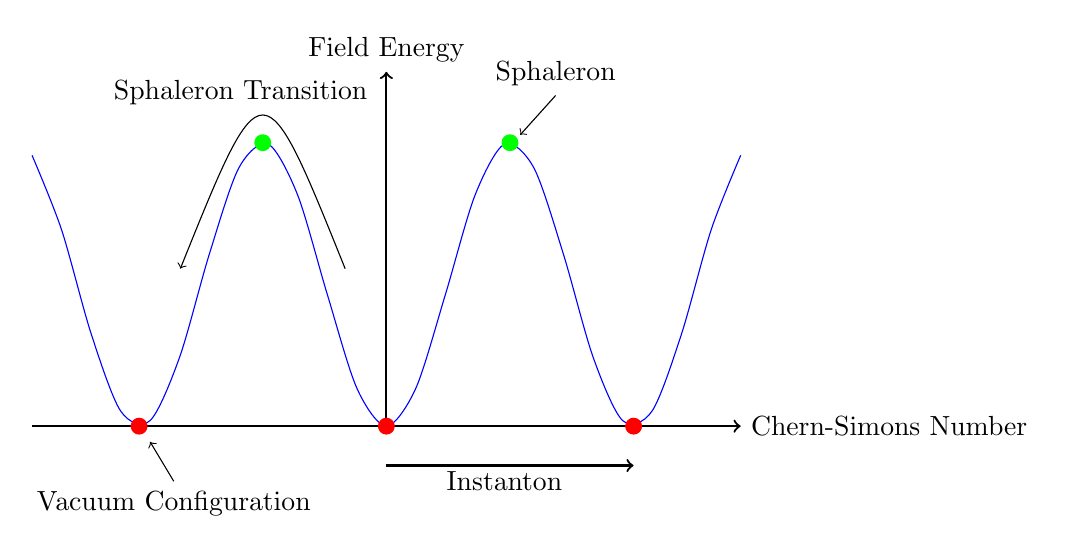
\begin{tikzpicture}
		\draw[thick,->] (-4.5,0) -- (4.5,0) node[anchor=west] {Chern-Simons Number};
		\draw[thick,->] (0,0) -- (0,4.5) node[anchor=south] {Field Energy};
		\draw[scale=1, domain=-4.5:4.5, smooth, variable=\x, blue] plot ({\x}, {1.8*(1 - cos(2 * \x r))});
		\foreach \x in {0,3.14,-3.14}
		\filldraw[color=red] (\x, 0) circle (0.1);
		\foreach \x in {3.14/2, -3.14/2}
		\filldraw[color=green] (\x, 1.8*2) circle (0.1);
		\draw[thick,->] (0.0, -0.5) -- (3.14, -0.5);
		\draw[->] (3.3 / 2 + 0.5, 1.8*2 + 0.5 + 0.1) node[anchor=south]  {Sphaleron} -- (3.4 / 2, 1.8*2 + 0.1) ;
		\draw[->] (-2.7, -0.7) node[anchor=north]  {Vacuum Configuration} -- (-3, -0.2) ;
		\node at (1.5, -0.7) {Instanton};
		\draw[->] (-3.14/6, 2) .. controls (-3.14 / 2, 1.8*2 + 1) .. (-3.14 + 3.14/6, 2) node[midway,above,xshift=-8]{Sphaleron Transition};
	\end{tikzpicture}
	\caption{Cartoon of the vacuum structure of a non-albelian gauge theory, which leads to the non-conservation of baryon and lepton numbers in the standard model.
		On the x-axis the Chern-Simons number is shown and on the y-axis the free-energy of the gauge field.
		The energy is sketched as a blue line. The vacuum-configurations are indicated by red dots and the sphaleron configurations by green ones. Sphaleron and instanton transitions are indicated by arrows from one vacuum state
		to the next.
	}
	\label{fig:sphaleron_cartoon}
\end{figure}


\chapter{Spontaneous Baryogenesis}
In this chapter we will discuss a possible mechanism which could implement baryogenesis. This mechanism is call spontaneous baryogenesis and is the topic of the rest of this thesis.

\section{Mechanism of Spontaneous Baryogenesis}

The mechanism of spontaneous baryogenesis was propose by Andreq Cohen and David Kapla in 1987 in \cite{COHEN1987251} and \cite{COHEN1988913}.
Their idea was to couple a scalar field $\phi$ to the baryon current $J_B$:
\begin{equation}
	\mathcal{L} = \frac{1}{2} (\partial \phi)^2 - V(\phi) - \frac{1}{f} \partial_\mu \phi J_B^\mu.
\end{equation}
If one considers the corresponding path-integral for the thermal theory, the time derivative in this coupling appears as a modification of the baryon chemical potential:
\begin{equation}
	\mu \to \mu_\mathrm{eff} = \mu + \frac{\dot{\phi}}{f}.
\end{equation}
This in turn modifies the equilibrium abundance of baryons, depending on the sign of $\dot{\phi}$.
In a cosmological setting, a scalar field is frozen until its mass exceeds the Hubble-friction (see \ref{sec:motion_of_the_axion_field} for details on this). The initial fast-roll motion creates baryons. Then the successive oscillations create baryons and antibaryons in alternation canceling each other, without creating a net baryon number.
There are different ways to create an concrete implementation of spontaneous baryogenesis.
The one we will look at in this thesis is using axions.
Axions have couplings the topological terms like
\begin{equation}
	 \sim \phi(t) F \tilde{F}.
\end{equation}
From eq. \eqref{eq:B_and_L_current_equations} we can see that this creates a direct coupling to the lepton current.
Then, by the means of sphalerons (see section \ref{sec:baryogenesis_in_the_standard_model}), the leptons are converted into baryons.

In ref. \cite{Domcke:2020kcp_Generic_Couplings} the authors pointed out that a direct coupling to the lepton or baryon current is not necessary for successful baryogenesis.
Instead the creation of some charge X deviating from the equilibrium value, leeds to a non-vanishing baryon number if the reactions which equilibrate the charge X back, are violating baryon number. Hence in the process a net baryon number is created.
Let us discuss this on an abstract example in more detail.
We are considering two charges $Q_1$ and $Q_2$. The baryon number is given by the linear combination
\begin{equation}
	B = Q_1 + Q_2.
\end{equation}
Our toy theory contains two interactions: $O_1$, which changes $Q_1$ by $-1$ and $Q_2$ by $+1$ and $O_2$, which changes $Q_1$ by $+1$. In equations, the current equations for this theory are:
\begin{align}
	\partial_\mu J_1^\mu &= O_2 - O_1 \\
	\partial_\mu J_2^\mu &= O_1 \nonumber.
\end{align}
Hence the current equation for the baryon current reads
\begin{equation}
	\partial_\mu J_B^\mu = O_2.
\end{equation}
The mechanism discussed so far would work by coupling the scalar field to the operator $O_2$, leading to a direct coupling of the scalar field to the baryon current. But in this example we couple it to $O_1$.
This coupling biases the value of $Q_2 - Q_1$ away from the previous vanishing equilibrium value.
At the same time, the the operator $O_2$ will lead to a relaxation of $Q_1$ toward its vanishing equilibrium value. In doing so it will violate also $B = Q_1 + Q_2$ as it doesn't change $Q_2$. Once this reaction freezes out, $B$ is conserved. Then $O_2$ will lead $Q_2 - Q_1$ to obtain its new vanishing equilibrium value with a non-vanishing $B$.
A cartoon of this process is shown in fig. ????? TODO

Why is this process called \emph{spontaneous} baryogenesis?
This is because the amount and also if baryons or antibaryons are generated depends on the initial value of the scalar field.
If in the UV-completion this scalar arises as the (pseudo-)Goldstone boson of the spontaneous symmetry breaking (SSB) of a complex field $\Phi$, then the initial values of $\phi$ are distributed evenly from the SSB, hence the name spontaneous baryogenesis.

Finally we have to find a way to compute the final asymmetry.
A simple approach is using Boltzmann equations. For example if we couple
the axion field directly to the lepton current and we have lepton number violating interaction in the thermal plasma mediated by the Weinberg operator
\begin{equation}
	???????
\end{equation}
then the Boltzmann equation reads:
\begin{equation}
	??????
\end{equation}
This equation was used in ref. \cite{Kusenko_2015_Axion_Leptogenesis}.
However we would like to have a complete set of equations considering all standard model charges. The equation above assumes that these charges are all in equilibrium.
Moreover this approach has the problem that it depends on the field basis.
This problem was pointed out by ref. \cite{Shi_2015_Basis_Invariance_chemical_equilibrium}.
If we would start with an axion coupling to the weak sphaleron $a F \tilde{F}$, this Boltzmann equation is not correct. As this coupling is not directly modifying the lepton chemical potential. For this one needs a coupling to the lepton current.
To introduce a coupling to the lepton current from this coupling, one needs to do a field redefinition depending on the axion field. This would also change the fields in the Weinberg operator, introducing a coupling within the Weinberg operator, modifying its rate. While one could compute a rate for the Weinberg operator including the axion dependence and solve for the asymmetry correctly, its more fruitful to use a set of basis independent equations.
This was done in .ref \cite{Domcke:2020kcp_Generic_Couplings}, where the authors developed a formalism based on linear-response theory which can describe the equilibration of charges by interaction and generation of charges from coupling to an axion field in a basis independent way for generic couplings. We will now recap their derivation.

\section{Transport Equation I: Derivation}
The following derivation of the transport equation is taken from  \cite[appendix B]{Domcke:2020kcp_Generic_Couplings}.

We start from the current (continuity) equation for the charges $Q_i$ with current $J_i^\mu$. These charges are changed by interaction $O_\alpha$ by $n_i^\alpha$:
\begin{equation}
	\label{eq:current_eq}
	\partial_\mu J_i^\mu = \sum_\alpha n_i^\alpha O_\alpha
\end{equation}
This equation is directly derived from the Lagrangian of the system and should be taken as an operator valued equation in the context of finite temperature QFT. We are working in the Heisenberg picture, where the states and the density matrix do not evolve with time but the observables do.
We want to take the expectation value in the grand-canonical ensemble as particle numbers are not conserved:
\begin{equation}
	\label{eq:current_eq_expectation_value}
	\partial_t \langle J_i^0 \rangle_{\mathrm{GC}} = \sum_\alpha n_i^\alpha \langle O_\alpha \rangle_{\mathrm{GC}}
\end{equation}
%The density matrix operator for the grand-canonical ensemble is given by
%\begin{equation}
%	\rho_\mathrm{GC} = \frac{e^{- (H - \sum_i \mu_i Q_i) / T}}{\operatorname{Tr} \left[ e^{- (H - \sum_i \mu_i Q_i) / T} \right] }.
%\end{equation}
We are going to evaluate these expectation values in linear-response theory.
For this we take $H_s \equiv \sum_i \mu_i Q_i$ as a perturbation to the Hamiltonian of the system.
Here the $\mu_i$ are the sources, which change slowly compared to the charges $Q_i$.
Let us first derive the equation for linear perturbation theory in general and then apply is first to the perturbation by chemical potentials $\mu_i$ and then to the perturbation by the classical axions field $a(t)$.
We work in the interaction-picture, where the time-evolution of the density matrix $\rho(t)$ of the system is given by
\begin{equation}
    \rho(t) = U(t) \rho_0 U^{-1}(t).
\end{equation}
The interaction-picture time-evolution operator $U(t)$ is given by
\begin{equation}
    U(t) = T \, \exp \left[ - i \int_{-\infty}^t  \mathrm{d} t' H_s(t') \right].
\end{equation}
We now evaluate an arbitrary observable $A_i$ with this density matrix in linear order of perturbation theory:
\begin{align}
    \langle A_i \rangle &= \operatorname{Tr} \left[ \rho(t) A_i(t) \right] \nonumber \\
    &= \operatorname{Tr} \left[ U(t) \rho_0 U^{-1}(t) A_i(t) \right] \nonumber \\
    &= \operatorname{Tr} \left[ \rho_0 U^{-1}(t) A_i(t) U(t) \right] \nonumber \\
    &\approx \operatorname{Tr} \left[ \rho_0 (1 + i \int_{-\infty}^t \mathrm{d} t' H_s(t')) A_i(t) (1 - i \int_{-\infty}^t \mathrm{d} t' H_s(t')) \right] \nonumber \\
    &\approx \operatorname{Tr} \left[ \rho_0 (A_i(t) + i \int_{-\infty}^t \mathrm{d} t' [H_s(t'), A_i(t)] ) \right] \nonumber \\
    &= \langle A_i \rangle_c + i \int_{-\infty}^t \mathrm{d} t' \langle [H_s(t'), A_i(t)] \rangle_c \nonumber \\
    &= \langle A_i \rangle_c + i \int_{-\infty}^t \mathrm{d} t' \langle [\sum_j \phi_j(t') A_j(t'), A_i(t)] \rangle_c  \nonumber \\
    &= \langle A_i \rangle_c + i \sum_j \int_{-\infty}^t \mathrm{d} t' \phi_j(t') \langle [A_j(t'), A_i(t)] \rangle_c
\end{align}

Now we can apply this to the chemical potentials.
We want to take the exception values of the interaction operators $O_\alpha$ in eq. \eqref{eq:current_eq_expectation_value}.
Here the chemical potentials $\mu_i$ are the sources and they are coupled to the charges $Q_i$.
Hence the linear response equations reads
\begin{equation}
	\langle O_\alpha(t, x) \rangle = i \sum_j \int_{-\infty}^t \mathrm{d} t' \mu_j(t') \langle [Q_j(t'), O_\alpha(t, x)] \rangle_c.
\end{equation}
Here we have used that $\langle O_\alpha(t) \rangle_c = 0$.
Now the are going to insert the charges in terms of the time component of the four-current:
\begin{equation}
	Q_i(t) = \int \mathrm{d}^3 x J^0_i(t, x)
\end{equation}
and insert a dummy integration to write the equation in terms of the time derivative of the charge density $\dot{J^0_i}$ and finally replace it with the right-hand-side of the current eq. \eqref{eq:current_eq}:
\begin{align}
	\langle O_\alpha(t, x) \rangle &= i \sum_j \int_{-\infty}^t \mathrm{d} t' \mu_j(t') \langle [\int \mathrm{d}^3 x' J^0_j(t', x'), O_\alpha(t, x)] \rangle_c \nonumber \\
	&= i \sum_j \int_{-\infty}^t \mathrm{d} t' \int \mathrm{d}^3 x'  \mu_j(t') \langle [\int^{t'}_{-\infty} \ \mathrm{d} t'' \frac{\partial}{\partial t''} J^0_j(t'', x'), O_\alpha(t, x)] \rangle_c \nonumber \\	
	&= i \sum_j \int_{-\infty}^t \mathrm{d} t' \int \mathrm{d}^3 x'  \mu_j(t') \langle [\int^{t'}_{-\infty} \ \mathrm{d} t'' \sum_\beta n^\beta_j O_\beta(t'', x'), O_\alpha(t, x)] \rangle_c \nonumber \\
	&= i \sum_{j, \beta} \int_{-\infty}^t \mathrm{d} t' \int \mathrm{d}^3 x' \int^{t'}_{-\infty} \ \mathrm{d} t'' \mu_j(t') n^\beta_j \langle [ O_\beta(t'', x'), O_\alpha(t)] \rangle_c
\end{align}
Finally we use the fact that the chemical potential changes slowly compared to the charges
\begin{equation}
	\langle O_\alpha(t, x) \rangle = i \sum_{j, \beta} \mu_j(t) n^\beta_j  \int_{-\infty}^t \mathrm{d} t' \int \mathrm{d}^3 x' \int^{t'}_{-\infty} \ \mathrm{d} t'' \langle [ O_\beta(t'', x'), O_\alpha(t, x)] \rangle_c.
\end{equation}
This equation can now be expressed in terms of the spectral functions 
\begin{equation}
	G_{\alpha \beta}(t - t', x - x') = \langle [ O_\alpha(t, x), O_\beta(t', x')] \rangle_{c}
\end{equation}
\begin{equation}G_{\alpha \beta}(\omega, p) = \int \mathrm{d}^4 x \, e^{i \omega t - i p \cdot x} G_{\alpha, \beta}(t, x)
\end{equation}
\begin{equation}G_{\alpha \beta}(t, x) = \int \frac{\mathrm{d}^3 x \, \mathrm{d} t}{2 \pi} \, e^{- i \omega t + i p \cdot x} G_{\alpha \beta}(\omega, p)
\end{equation}
%


% THIS IS FROM THE PAPER WHICH I DONT UNDERSTAND
% \begin{align}
% 	\mathcal{H}(t, \mathbf{x}) &= \varepsilon \int_{- \infty}^t \, \mathrm{d} t' e^{\varepsilon (t' - t)} \sum_i \mu_i J_i^0(t', \mathbf{x}) \nonumber \\
% 	&= \sum_i \mu_i J_i^0(t, \mathbf{x}) - \int_{- \infty}^t \, \mathbf{d} t' e^{\varepsilon (t' - t)} \sum_i \mu_i \sum_\alpha n_i^\alpha O_\alpha(t' , \mathbf{x})
% \end{align}
%
% \begin{align}
% 	\frac{\mathrm{d}}{\mathrm{d} t} \mathcal{H} = \varepsilon \sum_i \mu_i J_i^0(t, \mathbf{x}) - \varepsilon^2 \int_{- \infty}^t \, \mathrm{d}t' e^{\varepsilon (t' - t)} \sum_i \mu_i J_i^0(t', \mathbf{x}) \to 0
% \end{align}
%
% \begin{align}
% 	\rho \sim e^{- (H - \int \mathrm{d}^3 x \mathcal{H}) / T} = e^{-(H - \sum_i \mu_i Q_i) / T + X}
% \end{align}
%
% \begin{equation}
% 	X = - \sum_{i, \alpha} \frac{\mu_i}{T} n_i^\alpha \int_{- \infty}^t \, \mathrm{d}^4 x' e^{\varepsilon(t' - t)} O_\alpha(x')
% \end{equation}
%
% Pertubative expansion of $\rho$ in a series of $X$:
% \begin{equation}
% 	\rho \approx \left[ 1 + T \int_0^{1/T} \, \mathrm{d} \tau e^{-(H - \sum_i \mu_i Q_i) \tau} X e^{(H - \sum_i \mu_i Q_i) \tau} - \langle X \rangle_\mathrm{GC}  \right] \rho_\mathrm{GC}
% \end{equation}
%
% \begin{equation}
% 	\langle Q_\alpha \rangle = 0
% \end{equation}
%
%
% \begin{equation}
% 	\langle O_\alpha \rangle_\mathrm{GC} = \sum_{j, \beta} n_j^\beta \frac{\mu_j}{T} \int_{- \infty}^t \, \mathrm{d}^4 x' e^{\varepsilon (t' - t)} T \int_{0}^{1/T} \, \mathrm{d} \tau I
% \end{equation}
%
% \begin{align}
% 	I &= \left\langle O_\alpha(x) \left( e^{-(H - \sum_i \mu_i Q_i) \tau} O_\beta(x') e^{(H - \sum_i \mu_i Q_i) \tau} - \langle O_\beta(x') \rangle_\mathrm{GC} \right)  \right\rangle_{\mathrm{GC}} \nonumber \\
% 	&= \left\langle O_\alpha(x) \left( O_\beta(t' + i \tau, \mathbf{x}') - \langle O_\beta(x') \rangle_\mathrm{C} \right) \right\rangle_\mathrm{C} \nonumber \\
% 	&= \int_{- \infty}^{t'} \, \mathrm{d} t'' \left\langle O_\alpha(x) \frac{\mathrm{d}}{\mathrm{d} t''} O_\beta(t'' + i \tau, \mathbf{x}') \right\rangle_{\mathrm{C}}
% \end{align}
%
% \begin{equation}
% 	\langle O_\alpha \rangle_\mathrm{GC} = \sum_{j, \beta} n_i^\beta \mu_j \int_{- \infty}^t \, \mathrm{d}^4 x' e^{\varepsilon(t' - t)} \int_{- \infty}^{t'} \, \mathrm{d} t'' i \langle [ O_\alpha(x), O_\beta(t'', \mathbf{x}')] \rangle_\mathrm{C}
% \end{equation}
%
% Kubo-Martin-Schwinger Relation:
%
% \begin{align}
% 	\langle O_\alpha(x) O_\beta(t'' + i/T, \mathbf{x}') \rangle &= \operatorname{Tr} [ \rho_C O_\alpha(x) e^{- H / T} O_\beta(t'', \mathbf{x}') e^{+ H / T}] \nonumber \\ &= \langle O_\beta(t'', \mathbf{x}') O_\alpha(x) \rangle_{\mathrm{C}}
% \end{align}
%
% Definition spectral function:
% \begin{equation}
% 	G^\rho_{\alpha, \beta}(x - x') = \langle [ O_\alpha(x), O_\beta(x')] \rangle_{\mathrm{C}}
% \end{equation}
%
% Fourier transform of the real space spectral function:
% \begin{equation}
% 	G^\rho_{\alpha, \beta}(\omega, \mathbf{p}) = \int \mathrm{d}^4 x \, e^{i \omega t - i \mathbf{p} \cdot \mathbf{x}} G^\rho_{\alpha, \beta}(x)
% \end{equation}
%
% \begin{equation}
% 	\langle O_\alpha \rangle_\mathrm{GC} = \sum_{j, \beta} n^\beta_j \mu_j \lim_{\varepsilon \searrow 0} \int \frac{\mathrm{d} \omega}{\omega} \frac{1}{\omega - i \varepsilon} \frac{1}{i \varepsilon} G^\rho_{\alpha, \beta}(\omega, \mathbf{0}) = \sum_{j, \beta} n^\beta_j \frac{\mu_j}{T} \frac{T G^\rho_\alpha(\omega, \mathbf{0})}{2\omega} \big|_{\omega = 0}
% \end{equation}
%
% \begin{equation}
% 	\dot{q}_i = - \sum_j \sum_\alpha \Gamma_\alpha n_i^\alpha n_j^\alpha \frac{\mu_j}{T}
% \end{equation}
%
% Axion source term:
%
% \begin{equation}
% 	\mathcal{L}_{\mathrm{int}, \beta} = - \frac{a}{f} O_\beta
% \end{equation}
%
% \begin{equation}
% 	H(t) \to \tilde{H}(t) = H(t) + \frac{a(t)}{f} \int \mathrm{d}^3 x  O_\beta(t, \mathbf{x})
% \end{equation}
%
% \begin{equation}
% 	O_\alpha(t, \mathbf{x})|_{a/f} - O_\alpha(t_0, \mathbf{x}) = i \int_{t_0}^{t} \mathrm{d} t' [\tilde{H}(t'), O_\alpha(t', \mathbf{x})|_{a / f}]
% \end{equation}
%
% \begin{equation}
% 	\langle O_\alpha(t, \mathbf{x})|_{a/f} \rangle_{\mathrm{GC}} - \langle O_\alpha(t_0, \mathbf{x}) \rangle_{\mathrm{GC}} = i \int_{t_0}^{t} \mathrm{d} t' \langle [\tilde{H}(t'), O_\alpha(t', \mathbf{x})|_{a / f}] \rangle_{\mathrm{GC}}
% \end{equation}
%
%
% \begin{align}
% 	& \langle O_\alpha(t, \mathbf{x})|_{a/f} \rangle_{\mathrm{GC}} - \langle O_\alpha(t_0, \mathbf{x}) \rangle_{\mathrm{GC}} = \nonumber \\  & i \int_{t_0}^{t} \mathrm{d} t' \langle [H(t'), O_\alpha(t', \mathbf{x})|_{a / f}] \rangle_{\mathrm{GC}} + \frac{a(t')}{f} i \int_{t_0}^{t} \mathrm{d} t' \langle [O_\beta(t', \mathbf{x}'), O_\alpha(t', \mathbf{x})|_{a / f}] \rangle_{\mathrm{GC}}
% \end{align}
%
% \begin{align}
% 	i \int_{t_0}^{t} \mathrm{d} t' [H(t'), O_\alpha(t', \mathbf{x})|_{a / f}] &\approxeq i \int_{t_0}^{t} \mathrm{d} t' \langle [H(t'), O_\alpha(t', \mathbf{x})] \rangle_{\mathrm{GC}} + i \int_{t_0}^{t} \mathrm{d} t' \langle [H(t'), O_\alpha(t', \mathbf{x})|_{a / f}] \rangle_{\mathrm{C}} \nonumber \\ &= \langle O_\alpha(x) \rangle_{\mathrm{GC}} - \langle O_\alpha(t_0, \mathbf{x}) \rangle_{\mathrm{GC}}
% \end{align}
%
% \begin{align}
% 	\langle O_\alpha(x)|_{a/f} \rangle_{\mathrm{GC}} - \langle O_\alpha(t, \mathbf{x}) \rangle_{\mathrm{GC}} &\approxeq - i \int_{-  \infty}^t \mathrm{d}^4 x' \langle [ O_\alpha(x), O_\beta(x') ] \rangle_{\mathrm{C}} \frac{a(t')}{f} \nonumber \\ &= - i \int_{-  \infty}^t \mathrm{d}^4 x' G^\rho_{\alpha \beta}(x - x') \frac{a(t')}{f}
% \end{align}
%
% Axion moves slowly compared to reaction rates in the thermal plasma:
% \begin{equation}
% 	a(t') \approx a(t) + \dot{a}(t) (t' - t)
% \end{equation}
%
% Constant part:
% \begin{equation}
% 	- i \frac{a_0}{f} \int_{-  \infty}^t \mathrm{d}^4 x' G^\rho_{\alpha \beta}(x - x') = - i \frac{a_0}{f} \operatorname{Pv} \int \frac{\mathrm{d} \omega}{2\pi} \frac{1}{\omega} G^\rho_{\alpha \beta} (\omega, \mathbf{0})
% \end{equation}
%
% Derivative part:
% \begin{align}
% 	- i \frac{\dot{a}}{f} \int_{-  \infty}^t \mathrm{d}^4 x' G^\rho_{\alpha \beta}(x - x') &= - i \frac{\dot{a}}{f} \int_{-  \infty}^t \mathrm{d} t' \int \frac{\mathrm{d} \omega}{2\pi} e^{- i \omega (t - t')} \partial_\omega G^\rho_{\alpha \beta}(\omega, \mathbf{0}) \nonumber \\
% 	&= - i \frac{\dot{a}}{f} \lim_{\varepsilon \searrow 0} \int \frac{\mathrm{d} \omega}{2\pi i} \frac{1}{\omega - i \varepsilon} \partial_\omega G^\rho_{\alpha \beta}(\omega, \mathbf{0}) \nonumber \\
% 	&= \frac{\dot{a} / f}{T} \Gamma_\alpha \delta_{\alpha \beta}
% \end{align}


\begin{table}[h]
	content...
\end{table}


\begin{table}
	content...
\end{table}

\section{Transport Equation II: Dynamics}


% \section{Properties and Analytical Results}

\chapter{Motion of the Axion Field}
\label{sec:motion_of_the_axion_field}

In this chapter we will discuss the models for axion-like fields and their cosmological dynamics.
An overview of cosmological axion fields can be found in \cite{MarshAxionCosmo}.
First let us discuss some generalities common to all models.
We start from the action of (multiple) scalar fields $\phi_i$ on some background with metric $g$:
\begin{equation}
	S[\phi] = \int \mathrm{d}^4 x \sqrt{-g} \left[- \frac{1}{2} (\partial \phi)^2 - V(\phi) \right].
\end{equation}
The corresponding equation of motion reads:
\begin{equation}
	\label{eq:klein_gordon_general_background}
	\Box \phi \equiv \frac{1}{\sqrt{-g}} \partial_\mu \sqrt{-g} g^{\mu \nu} \partial_\nu \phi = \frac{\partial V(\phi)}{\partial \phi}.
\end{equation}
Now we are only interessted in the FLRW metric discussed in section \ref{sec:dynamics_of_the_examsion_of_the_universe}.
Let us compute the determinant of the metric
\begin{equation}
	g = \det g_{\mu \nu} = -1 \cdot \frac{a(t)^2}{1 - kr^2} \cdot a(t)^2 r^2 \cdot a(t)^2 r^2 \sin^2 \theta = - a(t)^6 f(\mathbf{x})
\end{equation}
as well as the box operator defined in eq. \eqref{eq:klein_gordon_general_background} for the metric:
\begin{align}
	    \Box \phi
	    &= - \frac{1}{\sqrt{a(t)^6 f(\vec{x})}} (\partial_t \sqrt{ a(t)^6 f(\vec{x}) }) \dot{\phi} - \ddot{\phi}
	    = - \frac{\partial_t a(t)^3}{a(t)^3} \dot{\phi} - \ddot{\phi} \nonumber \\
	    &= - \frac{\dot{a}(t) \cdot 3 a(t)^2}{a(t)^3} \dot{\phi} - \ddot{\phi}
	    = - 3 \frac{\dot{a}}{a} \dot{\phi} - \ddot{\phi}
	    = - 3H \dot{\phi} - \ddot{\phi}.
\end{align}
This gives us the equation of motion for scalar fields in an expanding universe:
\begin{equation}
	\ddot{\phi} + 3 H \dot{\phi} - \nabla^2 \phi / a(t)^2 + V'(\phi) = 0.
\end{equation}
In this thesis we assume that all fields are homogeneous after inflation and hence neglect the spacial derivatives of the Laplacian.

\section{ALP Realignment}
This model is the simplest model possible, which is a generic scalar field with mass $m_a$. Its Lagrangian is given as:
\begin{equation}
	\mathcal{L} = \frac{1}{2} \left( \partial_\mu \phi \right)^2 - \frac{1}{2} m_a^2 \phi^2.
	\label{eq:L_alp}
\end{equation}
The resulting equation of motion reads:
\begin{equation}
	\ddot{\phi} + 3 H \dot{\phi} + m_a^2 \phi = 0
\end{equation}

approximation for early times \cite[appendix A]{early_scalar_field_dynamics_PhysRevD.84.123506}:
\begin{equation}
	\label{eq:scalar_field_early_times_eom}
	c H \dot{\phi} \simeq - \frac{\partial V}{\partial \phi}
\end{equation}

move this formula maybe in fundamentals of cosmology section
\begin{equation}
	\frac{\dot{H}}{H^2} = - \frac{3(w + 1)}{2}
\end{equation}

In radiation domination we find $c = 5$.
Taking the derivative of \eqref{eq:scalar_field_early_times_eom} yields
\begin{equation}
	c \simeq 3 - \frac{\dot{H}}{H^2} - \frac{V''}{c H^2}
	= 3 + \frac{3(w + 1)}{2} - \frac{V''}{c H^2}
\end{equation}
Hence $c$ is constant as long as
\begin{equation}
	\frac{V''}{c H^2} \ll 1,
\end{equation}
holds.
Plugging in the harmonic potential for the ALP model:
\begin{equation}
	\dot{\phi} \simeq - \frac{1}{5 H} \frac{\partial V}{\partial \phi} = - \frac{1}{5 H} m_a^2 \phi
\end{equation}
as long as
\begin{equation}
	\frac{m_a^2}{c H^2} \ll 1 \implies m_a \ll c H
\end{equation}
The threshold of this equation is defined as $H_\mathrm{osc}$.
Once this condition is violated ($H \ll H_\mathrm{osc}$) we obtain a WKB-like solution for the ALP model:

\begin{equation}
	\phi = f_a t^{-1/2} \sin(m_a t + \delta)
\end{equation}


\begin{figure}[h]
    \includegraphics[width=\linewidth]{../../transport_eq_in_time/plots/alp_realignment_field_evolution.pdf}
    \caption{Evolution of the axion field for standard misalignment of an ALP with the Lagrangian in eq. \eqref{eq:L_alp}. On the x-axis time is shown in units of the axion mass $m_a$ on a log-scale. On the y-axis the misalignment angle $\theta$ is shown. Different epochs of the evolution are annotated.}
\end{figure}

\section{Clockwork Theory Axions and Deformed Potentials}

Based on \cite{Deformed_potential_Bae_2019}
Details of derivation of the clockwork potential are from \cite{general_cont_clockwork_Choi_2018}.

\begin{equation}
	\mathcal{L} = \frac{f^2}{2} Z(\theta) (\partial_\mu \theta)^2 - \Lambda^4 U(\theta)
\end{equation}

\begin{equation}
	\phi(x) \equiv f \int_0^{\theta(x)} \mathrm{d} \theta \sqrt{Z(\theta)}
\end{equation}

\begin{equation}
	\ddot{\phi} + 3 H \dot{\phi} + \frac{\partial V}{\partial \phi}
\end{equation}

\begin{equation}
	V(\phi) = \Lambda^4 U[\theta(\phi)]
\end{equation}

\begin{equation}
	\frac{\partial V}{\partial \phi} = \frac{1}{\sqrt{Z}} \frac{\Lambda^4}{f} \frac{\partial U}{\partial \theta}
\end{equation}

\begin{equation}
	\frac{\partial^2 V}{\partial \phi^2} = \frac{\Lambda^4}{f^2} \frac{1}{Z} \left( \frac{\partial^2 U}{\partial \theta^2} - \frac{1}{2 Z} \frac{\partial Z}{\partial \theta} \frac{\partial U}{\partial \theta} \right)
\end{equation}



We start by assuming a flat and compactified extra-dimension with a coordinate $y$. The compactification is on $S_1 / \mathbb{Z}_2$ with fixed points $y = 0$ and $y = mR$ \footnote{In ref. \cite{general_cont_clockwork_Choi_2018} a general dilaton background is considered and our calculations correspond to $k_1 = k_2 = k_3 = 0$.}.
On this space-time we introduce an angular field $\theta(x, y)$.
\begin{equation}
	S = \frac{f_5^3}{2} \int \mathrm{d} x^4 \mathrm{d} y \left[ (\partial_\mu \theta)^2 - (\partial_y \theta - m \sin(\theta))^2 \right]
\end{equation}
The equation of motion is obtained by varying $\theta \to \theta + \delta \theta$. In particular we need to keep track of the term linear in $\partial_y$ as it
creates boundary terms while the other terms behave like in regular Euler-Lagrange equations:
\begin{equation}
	\partial_\mu \partial^\mu \theta + \partial_y^2 \theta + m^2 \cos \theta m \sin(\theta) (\delta(y) - \delta(y - \pi R)).
\end{equation}
We are interested in the low energy theory. For this we want to decompose the field into separation of variables Ansatz. Because the potential introduces a non-linearity into the equations, we do a field redefinition
\begin{equation}
	\varphi(x, y) = \tan(\theta(x, y) / 2).
\end{equation}
\begin{equation}
	\theta(x, y) = \sum_{n = 0}^\infty f_n(y) \chi_n(x)
\end{equation}
We call the $f_n(y)$ the mode functions.





We now do a field redefinition
\begin{equation}
	\varphi(x, y) = \tan(\theta(x, y) / 2)
\end{equation}
and the action reads
\begin{equation}
	S = - \frac{f_5^3}{2} \int \mathrm{d}^5 x \frac{4}{(1 + \varphi^2)^2} \left[ (\partial_\mu \varphi)^2 + (\partial_y \varphi - m \varphi)^2 \right].
\end{equation}
From this we can derive the equations of motion


\begin{equation}
	k_1 = k_2 = 0
\end{equation}







\begin{equation}
	f^2 = f_5^3 (1 - \varepsilon^2) / (2m)
\end{equation}

\begin{equation}
	Z = \frac{1}{\coth(\pi m R) - \cos(\theta)} \approx \frac{2}{1 + 2\varepsilon^2 - \cos(\theta)}
\end{equation}

\begin{equation}
	V = \frac{2 \Lambda^4}{1 + \frac{1}{u^2[\phi]}}
\end{equation}

\begin{equation}
	\varepsilon \equiv e^{- \pi m R}
\end{equation}

\begin{equation}
	M \equiv \frac{\Lambda^2}{f}
\end{equation}

\begin{equation}
	u[\phi] = e^{-\pi mR} \operatorname{sc} \big[ \frac{\phi}{2f} \big| 1 - \varepsilon^2 \big]
\end{equation}

$\operatorname{sc}[\cdot | \cdot]$ is a Jacobi elliptic function

\footnote{
See \url{https://en.wikipedia.org/wiki/Jacobi_elliptic_functions} for an overview.
\begin{equation}
	u = \int_0^\varphi \mathrm{d} \theta \frac{1}{\sqrt{1 - m \sin^2 \theta}}
\end{equation}
\begin{align}
	\operatorname{am}(u, m) &\equiv \varphi \\
	\operatorname{sn}(u, m) &\equiv \sin \operatorname{am}(u, m) \\
	\operatorname{cn}(u, m) &\equiv \cos \operatorname{am}(u, m) \\
	\operatorname{dn}(u, m) &\equiv \frac{\mathrm{d}}{\mathrm{d} u} \operatorname{am}(u, m) \\
	\operatorname{sc}(u, m) &\equiv \tan \operatorname{am}(u, m)
\end{align}
\begin{equation}
	2 \pi f_\mathrm{eff} \equiv 4 f K(1 - \varepsilon^2)
\end{equation}
$K(\cdot)$ is the complete elliptic integral of the first kind
\begin{equation}
	K(k) \equiv \int_0^1 \mathrm{d}t \frac{1}{\sqrt{(1 - t^2)((1 - k^2t^2))}}
\end{equation}
$F( \cdot | \cdot )$ is the incomplete elliptic integral of the first kind:
\begin{equation}
	F(\phi | k^2) \equiv \int_0^\varphi \mathrm{d} \theta \frac{1}{\sqrt{1 - k^2 \sin^2 \theta}}
\end{equation}
}

\begin{equation}
	\phi \approx \frac{\pi f_\mathrm{eff}}{\varepsilon} \frac{F(\theta/2 | - 1 / \varepsilon^2)}{K(1 - \varepsilon^2)} = \frac{2}{\varepsilon} f F(\theta / 2 | - 1 / \varepsilon^2)
\end{equation}

\begin{equation}
	\frac{\partial V}{\partial \phi} = 4 \frac{\Lambda^4}{f^2} \frac{\frac{\partial u}{\partial \phi} f}{u^3(1 + 1/u^2)^2}
\end{equation}

\begin{equation}
	\frac{\partial u}{\partial \phi} = \epsilon \frac{1}{2 f} \frac{\operatorname{dn}[\phi/2f|1 - \varepsilon^2]}{(\operatorname{cn}[\phi/2f|1 - \varepsilon^2])^2}
\end{equation}

\begin{equation}
	\dot{\theta} = \frac{\frac{1}{2M^2} \left| \frac{\partial V}{\partial \phi} \right| \dot{\phi} / f}{\left(\left(1 - \frac{V/f^2}{2M^2}\right) \frac{V / f^2}{2 M^2} \right)^{1/2}}
\end{equation}

\begin{equation}
	\frac{\partial^2 V}{\partial \phi^2} = 4 M^2 \left[ f^2 \frac{\partial^2 u}{\partial \phi^2} \frac{1}{u^3(1 + 1/u^2)^2} + f^2 \left( \frac{\partial u}{\partial \phi} \right)^2 \frac{4(1 + 1/u^2) - 3u^2(1 + 1/u^2)^2}{\left( u^3(1 + 1/u^2)^2 \right)^2} \right]
\end{equation}

\begin{equation}
	\frac{\partial^2 u}{\partial \phi^2} = \frac{\varepsilon}{4 f^2} \left[ 2 \operatorname{cn}(\phi/2f|1 - \varepsilon^2)^{-3} \operatorname{dn}(\phi/2f|1 - \varepsilon^2)^2 - (1 - \varepsilon^2) \operatorname{cn}(\phi/2f|1 - \varepsilon^2)^{-1} \right] \operatorname{sn}(\phi/2f|1 - \varepsilon^2)
\end{equation}


TODO:


\begin{figure}[h]
    \includegraphics[width=\linewidth]{../../transport_eq_in_time/plots/cw_potential.pdf}
    \caption{Plot of the deformed potentials of the clockwork axion model. On the x-axis the value of the canonical normalized field $\phi$ over the effective axion decay constant $f_\mathrm{eff}$ in the angular range $[-\pi, +\pi]$ is shown on a linear-scale. On the y-axis the value of the potential over the energy scale of the confining sector $2 \Lambda^4$ is show. The potential is shown for different values of the size of the extra dimension $mR$ indicated by the color of the plot lines. The corresponding value of $mR$ is shown on a colorbar on the right hand side.}
\end{figure}

\begin{figure}[h]
    \includegraphics[width=\linewidth]{../../transport_eq_in_time/plots/cw_field_evolution.pdf}
    \caption{Plot of the evolution of the clockwork axion field as a function of time on the x-axis in units for the inverse mass scale $1/M$ on a log-scale. The canonical field is shown on the y-axis in units of the decay constant $f$. The different epochs of the field evolution described in the main text are annotated and the final epoch of oscillations are shown as an inset plot.}
\end{figure}


\section{Multi Axion Systems}

\begin{equation}
	\mathcal{L} = \frac{1}{2} \sum_i \left( \partial_\mu \phi_i \right)^2 - \sum_i \Lambda_i^4 \left[ 1 - \cos \left( \sum_j Q_{i,j} \, \phi_j / f_j \right) \right]
\end{equation}

\begin{equation}
	\mathcal{L} = \frac{1}{2} \sum_i \left( \partial_\mu \phi_i \right)^2 - \frac{1}{2} \sum_i m_i^2 \phi_i^2 - \sum_{i, j}
	g_{i, j} \phi_i^2 \phi_j^2
\end{equation}

\begin{figure}[h]
    \includegraphics[width=\linewidth]{../../transport_eq_in_time/plots/multi_axion_canonical_field_evolution.pdf}
    \caption{}
\end{figure}

\begin{figure}[h]
    \includegraphics[width=\linewidth]{../../transport_eq_in_time/plots/multi_axion_mass_eigenstate_field_evolution.pdf}
    \caption{}
\end{figure}

\begin{figure}[h]
    \includegraphics[width=0.5\linewidth]{../../transport_eq_in_time/plots/multi_mass_eigenstate_configspacen.pdf}
    \includegraphics[width=0.5\linewidth]{../../transport_eq_in_time/plots/multi_axion_canonical_configspace.pdf}
    \caption{}
\end{figure}

\begin{figure}[h]
    \includegraphics[width=\linewidth]{../../transport_eq_in_time/plots/multi_axion_powerspectrum1.pdf}
    \includegraphics[width=\linewidth]{../../transport_eq_in_time/plots/multi_axion_powerspectrum2.pdf}
    \caption{}
\end{figure}






\chapter{Results}

\section{ALP Realignment}

\begin{figure}[h]
    \includegraphics[width=\linewidth]{../../transport_eq_in_time/plots/alp_paramspace.pdf}
    \caption{Contour plots of the obtained baryon asymmetry  for the ALP model (shown as the decimal logarithm relative to the observed asymmetry) for the different couplings ($a\tilde{F}F)$ on the left, $a\partial J$ in the middle and $a \tilde{G} G$ on the right as a function of the axion mass $m_a$ in GeV on the x-axis on a log-scale and of the inflaton decay rate in GeV on the y-axis on a log-scale (shown on the left-most plot on the left-hand-side). The reheating temperature $T_\mathrm{RH}$ corresponding to the inflaton decay rate is shown on the right most plot on the right hand side in GeV also on a log-scale. A red line indicates the points where the observed asymmetry is reached. The values of the axion decay constant $f_a$ and Hubble scale a the end of inflation $H_\mathrm{inf}$ are given in the title. All contour plots share the same colorbar, shown below the plots.}
\end{figure}

\begin{figure}[h]
    \includegraphics[width=\linewidth]{../../transport_eq_in_time/plots/alp_correct_f_a_curves.pdf}
    \caption{The curves where the observed baryon asymmetry is reached for the ALP model for different values of the axion decay constant $f_a$ for the different couplings ($a \tilde{F} F$ on the left, $a \partial J$ in the middle and $a \tilde{G} G$ on the right). The curves are shown in the inflaton decay rate $\Gamma_\mathrm{inf}$ (shown on the y-axis on a log-scale in GeV on the left-most plot) and axion mass $m_a$ (shown on the x-axis on a log-scale in GeV). Also the reheating temperature $T_{\mathrm{RH}}$ in GeV on a log-scale corresponding to the inflaton decay rate is shown on the right-most plot.
    Each curve is colored corresponding to the value of the axion decay rate used on a log-scale. The colorbar showing the corresponding $f_a$ value is displayed on the bottom.}
\end{figure}

\begin{figure}[h]
	\includegraphics[width=0.6\linewidth]{../../transport_eq_in_time/plots/alp_minimal_possible_m_a_and_Gamma_inf_vals.pdf}
	\caption{The minimal values of the axion mass $m_a$ (solid lines) and the inflaton decay rate  $\Gamma_\mathrm{inf}$ (dashed lines) in GeV where the observed baryon asymmetry is reached as a function of the axion decay constant $f_a$ in GeV which is shown on the x-axis in units of GeV and on a log-scale. The different couplings are shown in different colors ($a F \tilde{F}$ in blue, $a \partial J$ in orange, $a G \tilde{G}$ in green).}
\end{figure}

\begin{figure}[h]
    \includegraphics[width=\linewidth]{../../transport_eq_in_time/plots/alp_exploration_plot0.pdf}
    \caption{The contour plot in the middle row shows the obtained baryon asymmetry for the ALP model for the $a \tilde{F} F$ coupling with the axion mass $m_a$ in GeV on the x-axis on a log-scale and the inflaton decay rate $\Gamma_\mathrm{inf}$ in GeV on the y-axis on a log-scale. The asymmetry is shown as the decimal logarithm relative to the observed asymmetry. A red line indicates where the observed asymmetry is reached. On the top and bottom rows the time evolution for a few example points in the parameter space of the contour plot are shown. The parameter values for of the examples are indicated by arrows into the contour plot. Each time evolution plot consists of a plot of the value of the chemical potential of the B-L charge on a log-scale as a function of time (black line). While on the bottom a plot of the reaction rate for the creation of B-L charges (blue line, log-scale, axis on the left) and of the source from the axion (orange line, linear-scale, axis on the right) is shown.
    	Both the top and the bottom plots use the same time-axis on a log-scale. On the bottom the time is shown in units of the inverse inflaton decay rate $1/\Gamma_\mathrm{inf}$ and on the top in units of the inverse axion mass $1/m_a$.}
    \label{fig:alp_explorations_plot_aFF}
\end{figure}

\begin{figure}[h]
    \includegraphics[width=\linewidth]{../../transport_eq_in_time/plots/alp_exploration_plot1.pdf}
    \caption{Same as fig. \ref{fig:alp_explorations_plot_aFF} but for the $a \partial J$ coupling.}
\end{figure}

\begin{figure}[h]
    \includegraphics[width=\linewidth]{../../transport_eq_in_time/plots/alp_exploration_plot2.pdf}
    \caption{Same as fig. \ref{fig:alp_explorations_plot_aFF} but for the $a \tilde{G} G$ coupling.}
\end{figure}

\section{Clockwork Theory Axions}

\begin{figure}[h]
    \includegraphics[width=\linewidth]{../../transport_eq_in_time/plots/cw_m_phi_vs_mR_1.pdf}
    \caption{Contour plots of the $mR$ vs $m_\phi$ parameter space of the clockwork model for the different values of the inflaton decay rate $\Gamma_\mathrm{inf}$ (in the different rows, value denoted in the y-label on the left-most plot of each row) and the axion decay rate $f_a$ (in the different columns, value denoted in the x-label of the bottom plot if each column). Each contour plot has $mR$ on the y-axis on a linear scale shown on the left most plot of each row and $m_\phi$ in eV on the x-axis on a log-scale shown on the bottom plot of each column. In each plot the baryon asymmetry as the decimal logarithm relative to the observed baryon asymmetry is shown as green-blueish colored contour lines. The axion relic density as the decimal logarithm relative to the observed dark matter density is shown as red-yellowish  colored contour lines. The curves where the observed baryon asymmetry is reached is indicated by a solid black line. The curves where the dark matter density is reached is indicated by a dashed black line. The intersection of both lines is shown as a red dot. Below the plots the colorbars for the baryon asymmetry and the relic density contour lines are shown. In each plot a red colored region indicates the part of the parameter space where the axion would start oscillating before the end of inflation invalidating our model. A orange region shows the part where the clockwork axion would decay within the life-time of the universe. }
    \label{fig:clockwork_parameter_space_aFF}
\end{figure}

\begin{figure}[h]
    \includegraphics[width=\linewidth]{../../transport_eq_in_time/plots/cw_m_phi_vs_mR_2.pdf}
    \caption{Same as fig. \ref{fig:clockwork_parameter_space_aFF} but for the $a \partial J$ coupling.}
\end{figure}

\begin{figure}[h]
    \includegraphics[width=\linewidth]{../../transport_eq_in_time/plots/cw_m_phi_vs_mR_3.pdf}
    \caption{Same as fig. \ref{fig:clockwork_parameter_space_aFF} but for the $a G \tilde{G}$ coupling.}
\end{figure}

\begin{figure}[h]
    \includegraphics[width=\linewidth]{../../transport_eq_in_time/plots/cw_m_phi_vs_Gamma_inf.pdf}
    \caption{The clockwork axion parameter space contour plots of the baryon asymmetry as the decimal logarithm relative to the observed baryon asymmetry as a function the inflaton decay rate $Gamma_\mathrm{inf}$ in GeV on the y-axis on a log-scale and the axion mass $m_\phi$ in eV on the x-axis on a log-scale.
    Each row has a different coupling namely $a F \tilde{F}$ in the top row, $a \partial J$ in the middle row and $a G \tilde{G}$ in the bottom row. Each column has a different value of the size of the extra dimension $mR$ indicated on the x-label of the bottom plot of each column. Each plot has its own colorbar for the contour lines as the scales are very different for each plot. A red line is used to indicate the curves where the observed baryon asymmetry is reached.}
\end{figure}

\begin{figure}[h]
	\includegraphics[width=\linewidth]{../../transport_eq_in_time/plots/cw_exploration_plot.pdf}
	\caption{A contour plot of the clockwork axion mass $m_\phi$ vs size of the extra dimension $mR$ parameter-space is shown in the middle row. The baryon asymmetry is shown in green-blueish contour lines. The relic density is shown in red-yellowish contour lines. Both are shown are the decimal logarithm relative to the observed value. The red colored area indicates the part of the parameter-space where axion oscillates before the end of inflation and hence invalidates the model. The orange area indicates the that the axion decays within the life-time of the universe. In the top and bottom rows the time evolution of the processes corresponding to example points in the parameter space indicated by arrows is shown. Each of these plots consists of three subplots. On the left the evolution of the canonical clockwork field until the oscillations is shown. On the right the time evolution of the chemical potential over the temperature and the rate of B-L generation and the axion source as in fig. \ref{fig:alp_explorations_plot_aFF} are shown.}
\end{figure}

\section{Multi Axion Systems}

\chapter{Summery and Conclusion}


\appendix

\chapter{Some Appendix ....}

\cleardoublepage
%% Bibliographie. Das Argument muss der Name der BIBTeX-Datenbank stehen.
%% Ein Beispiel fuer eine solche Datenbank finden Sie in bthesis_datenbank.bib
\bibliography{bthesis_datenbank}

\chapter*{Acknowledgment}
I thank Doddy Marsh and Laura Covi for the supervison and the possibility to take half a year off for a health break. Also I thank my doctors and friends. You saved my life. Finally I thank .... for finding a lot of typos, grammar and spelling mistakes.

\end{otherlanguage}
%% Dieser Befehl MUSS am Ende stehen und erzeugt die Erklaerung ueber die
%% benutzten Mittel
\Declaration
\end{document}
